% fig:roadmap -- tensor factors (left) vs. operator subalgebras (right).
% Included at 0.92\textwidth (~15.2 cm); drawn at roughly that natural width.
\documentclass[tikz,border=4pt]{standalone}
\usepackage{lmodern}
\usepackage{amsmath,amssymb}
\usepackage{xcolor}
\usepackage{tikz}
\usetikzlibrary{arrows.meta,calc,decorations.pathmorphing}

\definecolor{boxblue}{HTML}{eef3fa}
\definecolor{boxgold}{HTML}{fbf3e3}
\definecolor{boxgreen}{HTML}{eaf6f0}
\definecolor{ruleblue}{HTML}{2b6cb0}
\definecolor{rulegold}{HTML}{b7791f}
\definecolor{rulegreen}{HTML}{1f8a5f}

\newcommand{\HH}{\mathcal{H}}
\newcommand{\M}{\mathcal{M}}
\begin{document}
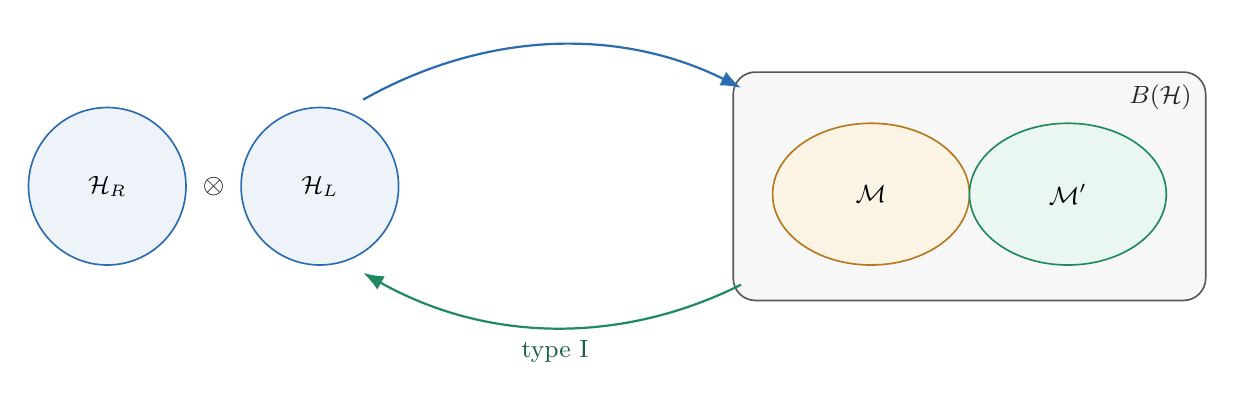
\begin{tikzpicture}[every node/.style={font=\small}, line width=0.6pt]

% ---------------- left: tensor product of two Hilbert spaces --------------
\begin{scope}[shift={(0,0)}]
  \draw[ruleblue, fill=boxblue] (-1.35,0) circle (1.0);
  \draw[ruleblue, fill=boxblue] ( 1.35,0) circle (1.0);
  \node at (-1.35,0) {$\HH_R$};
  \node at ( 1.35,0) {$\HH_L$};
  \node[font=\normalsize] at (0,0) {$\otimes$};
\end{scope}

% ---------------- right: subalgebras inside B(H) ---------------------------
\begin{scope}[shift={(9.6,0)}]
  \draw[gray!70!black, rounded corners=8pt, fill=gray!6] (-3.0,-1.45) rectangle (3.0,1.45);
  \node[anchor=north east, gray!30!black] at (2.95,1.42) {$B(\HH)$};
  \draw[rulegold, fill=boxgold] (-1.25,-0.1) ellipse (1.25 and 0.9);
  \draw[rulegreen, fill=boxgreen] (1.25,-0.1) ellipse (1.25 and 0.9);
  \node at (-1.25,-0.1) {$\M$};
  \node at ( 1.25,-0.1) {$\M'$};
\end{scope}

% ---------------- arrows ---------------------------------------------------
\draw[-{Latex[length=2.6mm]}, ruleblue, thick]
  (1.9,1.1) .. controls (3.5,2.0) and (5.2,2.0) .. (6.7,1.25);
\draw[-{Latex[length=2.6mm]}, rulegreen, thick]
  (6.7,-1.25) .. controls (5.2,-2.0) and (3.5,-2.0) .. (1.9,-1.1)
  node[pos=0.5, below=1pt, text=rulegreen!70!black] {type I};

\end{tikzpicture}
\end{document}
